\documentclass[fleqn]{jaes}

% Metadata Information
\jyear{2025}
\jmonth{October}

\usepackage{amsmath}\setlength{\mathindent}{10pt}
\DeclareMathAlphabet{\pazocal}{OMS}{zplm}{m}{n}
\SetMathAlphabet\pazocal{bold}{OMS}{zplm}{bx}{n}
\usepackage{bm}
\usepackage{xcolor}
\usepackage{hyperref}


\begin{document}

% Page heads
\markboth{MEIK\"AL\"AINEN AND DOE}{JAES TEMPLATE}


% Title portion
\title{Modeling underwater sound propagation}

%Author Info.
\authorgroup{
\author{OTTO AHONIEMI}, \author{HOCINE MONTENEZ}
AND \author{ATTE STENQVIST}
}

%Abstract
%An informative and self-contained abstract of 100 to 200 words must be provided. The abstract should mention the motivation, problem statement, approach, results, and implications of the work, usually with one or two sentences each. It is recommended that the abstract be written in a single paragraph without citing any references. The Journal of the Audio Engineering Society is a modern scientific journal supporting online publishing with colors and a graphical abstract. It is a hybrid journal publishing both Open Access and traditional papers, the latter being only available for subscribers, such as AES members. If a paper published in the Journal of the Audio Engineering Society has been made Open Access, it will have the OA logo next to it and will be freely downloadable from the AES E-Library by anyone, even if they are not an AES member or E-Library subscriber. This example abstract contains 149 words.
\abstract{%
}
\maketitle
%Head 1
% \section{INTRODUCTION}
% \subsection{Context}
% %What why
% %Why its more difficult than we expect snell, ssp, etc


% \subsection{Literature review}
% \begin{itemize}
%     \item SSP equation more precise/different conditions Atte 
%     \item Ray reflection on the seabed H
%     \item Transfer loss H
%     \item Impact of ray propagation on animals? Otto
%     \item Impact of fish on propagation? Otto
% \end{itemize}

% \begin{itemize}
%     \item ray based methods H
%     \item other blablabla based methods Otto
% \end{itemize}


% \section{METHODS="models"}
% \subsection{Dumb euler}

% \subsection{C-linear}
% \subsection{BellHop}

% \newpage
% \clearpage
\section{INTRODUCTION}

\subsection{Sound propagation in the ocean}
In ocean acoustics, sound is propagated using the ocean as a waveguide, limited between the surface and the seafloor. Within this waveguide, speed of sound varies due to density, which in the ocean is related to static pressure, salinity and temperature. Many different empirical formulas for calculating the speed of sound have been proposed \cite{Huang} with varying complexities and application ranges, but for most cases the simplified Medwin empirical formula can be used as a an approximation \cite{Jensen}, \cite{Lurton}. In the Medwin formula, speed of sound ($c$, in $m/s$) is calculated as 

\begin{equation}
\begin{split}
c &= 1449.2 + 4.6T - 0.055T^2 + 0.00029T^3 \\
  &\quad + (1.34 - 0.01T)(S-35) + 0.016z
\end{split}
\label{eq:speedofsound}
\end{equation}
where $t$ is the temperature, in $C$°; $S$ is the salinity, in parts per million and $z$ is the depth, in $m$. 

Due to the variety of temperature, salinity and depth in the oceans around the world, underwater sound propagation is strictly dependent on the \textit{sound speed profile} (SSP) that is used. A typical SSP in deep non-polar oceans has an unstable mixed layer near the surface and a stable, linearly increasing sound speed profile in the deep isothermal layer near the seafloor \cite{Jensen}. Between these regions exists the \textit{deep sound channel}, where the speed of sound reaches a minimum. The \textit{Munk profile}, is an idealized SSP showcased in Fig. \ref{fig:munk}, which contains many features of deep-water propagation and is often used for demonstrations of deep-water propagation.

For determining the sound propagation paths, speed of sound is treated in the same way the index of refraction is treated in optics. The refraction of the propagation direction changes as the speed of sound changes in accordance with \textit{Snell's law}, 

\begin{equation}
\frac{\cos{\theta}}{c}= p,
\label{eq:snellslaw}
\end{equation}

where $p$ is a constant $\theta$ is the ray angle and $c$ is the local speed of sound \cite{Lurton}. Sound rays will therefore bend towards regions with lower speed of sound. A demonstration of deep-water propagation paths using the Munk profile is shown in Fig \ref{fig:munk}.

\begin{figure*}
\centering
\centering
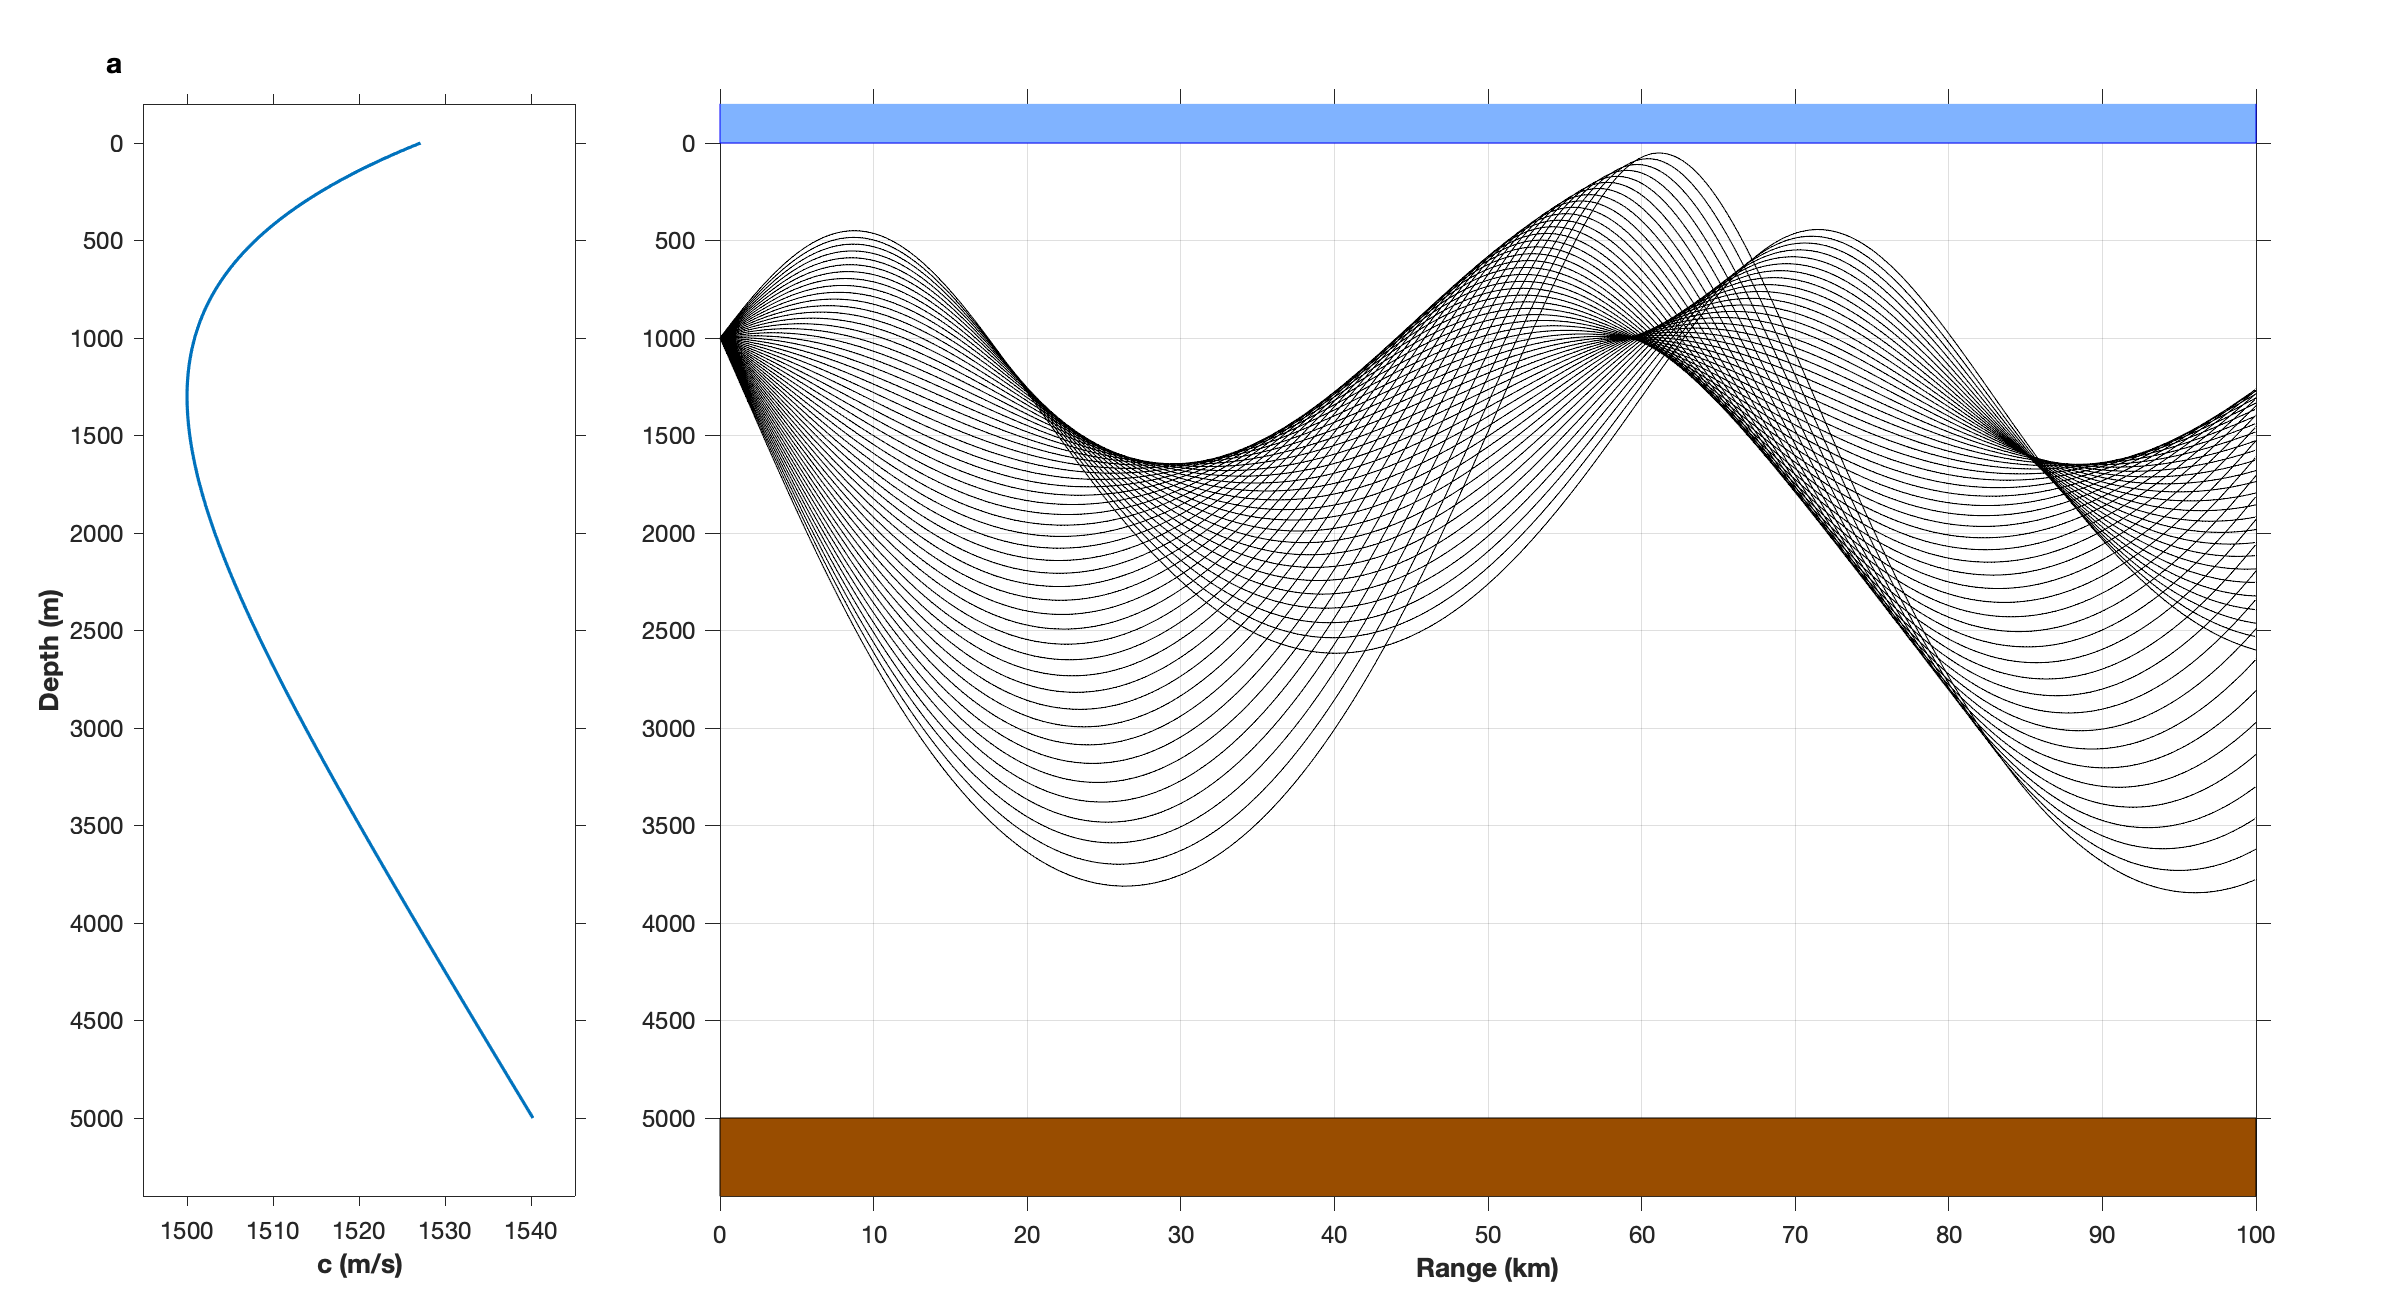
\includegraphics[trim=0cm 0.5cm 0cm 0.5cm, width=0.8\textwidth]{sspExample.png}
\caption{Munk sound speed profile (left) and sound propagation rays in Munk sound speed profile (right). Ray tracing using C-linear method.}
\label{fig:munk}
\end{figure*}

\subsection{Reflections}
At the surface and at the seabed of the ocean, the waves will experience reflections. In general, when the medium is not perfectly lossless, the local sound speed $c$ becomes complex, and the reflection coefficient is therefore also complex. Each reflection introduces both an amplitude loss and a phase shift. The reflection coefficient $\pazocal{R}$ and transmission coefficient $\pazocal{T}$ at an interface between two fluid media can be expressed in terms of their specific acoustic impedances $\pazocal{Z}_i = \rho_i c_i / \sin\theta_i$ as

\begin{equation}
\pazocal{R} = \frac{\pazocal{Z}_2 - \pazocal{Z}_1}{\pazocal{Z}_2 + \pazocal{Z}_1}
\quad\quad
\pazocal{T} = \frac{2\pazocal{Z}_2}{\pazocal{Z}_2 + \pazocal{Z}_1}.
\end{equation}

When the two media have similar acoustic impedance ($\pazocal{Z}_1 \approx \pazocal{Z}_2$), the reflection coefficient is almost zero. Conversely, when medium 1 has a much larger impedance than medium 1, the reflection coefficient is close to 1, meaning that most of the energy is reflected.

\subsubsection{Surface reflections}
At the interface, the difference in acoustic impedance between air and water is so large that almost total reflection occurs ($\pazocal{R} \approx 1$). The surface can therefore be approximated as a perfectly reflecting boundary. However, this assumption breaks down in agitated conditions when wind and waves generate bubbles that scatter and absorb acoustic energy, leading to non negligible reflection losses \cite{Jensen}. 

In deep water, this bending traps the acoustic energy, hence creating ray paths that travel long distances without ever touching the bottom and that only reflect from the surface. Such typical deep-water environments, where these effects are prominent, occur in all oceans at depths exceeding about 2000m \cite{Jensen}. In this case, sound propagation often occurs without significant bottom interaction, dominated instead by refraction and surface reflection.

\subsubsection{Bottom reflections}

Reflection from the ocean bottom is far more complex. Unlike the nearly perfect surface, the bottom is generally a lossy boundary composed of sediments and rock layers with variable density, sound speed, and attenuation. The impedance mismatch between water and seabed materials determines how much energy is reflected versus transmitted into the sediment.

Layered sediments further complicate this behavior, producing frequency- and angle-dependent reflection losses due to interference within the layers. Depending on the incident angle, thin or half-wavelength layers can be acoustically transparent, while quarter-wavelength layers can act as anti-reflecting coatings \cite{Jensen}.

\subsection{Transfer loss}
As waves travel through the water, their amplitude is progressively attenuated by two important effects: absorption and scattering. This attenuation is usually modeled by an exponential decay law with distance $x$:
\begin{equation}
    A = A_0 \exp (-\alpha x)
    \label{eq:attenuationdecay}
\end{equation}
where $A_0$ is the rms amplitude at $x=0$ and $\alpha$ is the attenuation factor.
The coefficient $\alpha$ has some dependence on frequency, temperature, pressure, salinity, and acidity. However, a simplified expression depending only on frequency is considered sufficiently accurate for most problems in ocean acoustics \cite{Jensen, urick1979}: 
\begin{equation}
    \alpha = \frac{1}{8.69} \big[ 3.3 \cdot 10^{-3} + \frac{0.11f^2}{1+f^2} + \frac{44f^2}{4100+f^2} + 3\cdot 10^{-4} f^2\big]
    \label{eq:attenuationfrequency}
\end{equation}
where $f$ is expressed in kHz and $\alpha$ in dB/km. Equation \ref{eq:attenuationfrequency} shows attenuation increases with frequency, such that low-frequency waves are only mildly attenuated, making them an highly effective for long-range underwater communication compared to electromagnetic waves. For example, a 100Hz acoustic signal would need to travel around 2200 km to be attenuated by -10dB.

\subsection{Volume scattering (fish)}

In addition to boundary interactions at the sea surface and seafloor, sound propagation in the ocean is affected by volume scattering from marine life within the water column. Volume scattering is characterized by a scattering cross section, defined as the ratio of scattered power to incident intensity on a unit volume. This scattering contributes to both attenuation of coherent acoustic signals and generation of reverberation that interferes with sonar detection.

At lower frequencies (below 10 kHz), fish with gas-filled swim bladders are the dominant volume scatterers \cite{Jensen}. The swim bladder presents a high acoustic impedance contrast with the surrounding tissue and seawater, causing strong backscattering. Above 20 kHz, smaller organisms such as zooplankton become the primary scatterers. The target strength of individual fish depends on fish size, swim bladder morphology, frequency, and orientation relative to the acoustic beam, with typical values ranging from $-$40 to $-$20 dB for individual fish at moderate frequencies \cite{Foote1983}. The swim bladder contribution accounts for 90-95\% of the backscattered energy.

Volume scattering strength generally decreases with depth at approximately 5 dB per 300 m, with a notable exception being the deep scattering layer (DSL). The DSL is a concentrated layer of marine organisms, primarily small fish and zooplankton, that migrate vertically in the water column following the diurnal cycle. This layer can produce scattering returns comparable in magnitude to those from physical boundaries \cite{Jensen}.

In acoustic propagation modeling, volume scattering introduces two main effects: attenuation of the coherent field through scattering loss, and generation of a diffuse reverberation field. The volume scattering strength $S_v$ is expressed in decibels and relates the scattered intensity to incident intensity per unit volume. For a layer of thickness $H$, the integrated column scattering strength $S_c$ can be computed by integrating the local volume scattering strength $s_v(z)$ over depth. These parameters are used in sonar performance prediction and acoustic propagation models for applications such as fisheries acoustics and marine mammal protection.

\subsection{Sound propagation models}
Underwater sound propagation can be described using several types of models, each based on different approximations of the acoustic wave equation. These models vary in their physical assumptions, numerical complexity, and suitability for particular frequency ranges or environmental conditions. This section briefly presents the most popular families of methods \cite{propagationmodels, Jensen}.

First, ray theory based models describe sound as energy traveling along discrete geometric paths, or rays. This approach is particularly effective when the acoustic wavelength is small compared to the scale of environmental variations, such as at high frequencies or over long distances. The use of ray-based models in the research community was motivated by their simplicity and computational efficiency. However, they neglect diffraction and interference effects, making them less commonly used when it comes to model low frequency phenomena\cite{hovem2019}.

Next, the wave equation can also be solved by using the separation of variables technique to isolate the vertical and horizontal directions. The vertical wave equation solutions are
normal modes, or eigenvalues, that can then be summed up in varying
fashion, depending upon the horizontal propagation, at the source and receiver to
generate the full acoustic field.
Each mode behaves like a standing wave in depth and propagates horizontally with its own phase speed. This approach is particularly suited for low-frequency and long-range propagation, as it can accurately describe the interference patterns between modes. The main drawback of normal mode models is that they become too computationally expensive at high frequencies\cite{propagationmodels}.

Finally, as most of the problems solved in ocean acoustics involve a one-way propagation (i.e. from source to receiver) separating the wave equation into incoming and outgoing solutions leads to the
Parabolic Equation (PE) method. PE models can account for refraction, diffraction, and scattering, which explains why they are so widely used and popular in the research community \cite{Jensen}. The PE computational
load increases with the square of the frequency and which generally limits its use to frequencies less than 1 kHz \cite{propagationmodels}.

In summary, each category of sound propagation model offers a different balance between accuracy, complexity and computational cost. The choice of the model is determined by the problem requirements.

\section{METHODS}
For this paper three different underwater sound propagation models were tested and reviewed. The models \textit{Geometric ray tracing} (described in Section 1.1) and \textit{c-linear} (described in Section 1.2) are simple ray-based methods implemented by the authors based on techniques represented in \cite{Jensen}. The \textit{Bellhop} model described in Section 1.3 is a more advanced beam tracing program implemented using open source code from \cite{Porter}.

\subsection{Geometric Ray Tracing}
In this project, the underwater acoustic propagation was first modeled using the geometric ray tracing, governed by Snell’s law. This simple method does not solve the full acoustic wave equation, but approximates the trajectories of sound waves as they travel through the horizontally stratified water environment. 

The environment is represented by a one-dimensional sound speed profile $c(z)$ that varies with depth $z$. 
A simple Munk-like profile \cite{Porter} was employed to approximate realistic ocean conditions:
\begin{equation}
    c(z) = c_0 \left[ 1 + \epsilon \left( \bar{z} - 1 + e^{-\bar{z}} \right) \right],
    \quad \text{where} \quad
    \bar{z} = \frac{2(z - z_0)}{z_0}.
\end{equation}
where $c_0 = 1500~\text{m/s}$ is the reference sound speed, $z_0 = 1300~\text{m}$ is the reference depth (the sound channel axis), and $\epsilon = 0.00737$ is a non-dimensional perturbation parameter controlling the strength of the sound speed variation. 

The trajectory of the ray is governed by the differential equations:
\begin{equation}
    \frac{dx}{ds} = \cos\theta \quad \quad
    \frac{dz}{ds} = \sin\theta,
    \label{eq: dsRelations}
\end{equation}
where $s$ is the arclength along the ray. The local angle $\theta$ can be recovered from Snell’s law:
\begin{equation}
    \theta(z) = \arccos\!\left(p\,c(z)\right),
\label{eq:arccosSnell}
\end{equation}
provided that $|p\,c(z)| \leq 1$, where $p$ is the Snell's law constant.

\subsubsection{Numerical Integration}

The ray paths were computed by discretizing the arclength $s$ into small steps of size $\Delta s$ and updating the horizontal and vertical positions as
\begin{align}
    x_{n+1} &= x_n + \Delta s \cos\theta_n, \\
    z_{n+1} &= z_n + \Delta s \sin\theta_n,
\end{align}
where $\theta_n$ is evaluated at the current depth using Snell’s law. 

At each step, reflections from the sea surface and bottom boundaries were handled by reversing the vertical direction of propagation:
\begin{equation}
    \sin\theta_{n+1} = -\,\sin\theta_n,
    \label{Perfectreflection}
\end{equation}
whenever the ray reached $z = 0$ (surface) or $z = z_{\text{max}}$ (bottom).

\subsubsection{Source and Receiver Configuration}

A point source was positioned at depth $z_s = 1000~\text{m}$, and multiple rays were launched at different initial grazing angles $\theta_0$ spanning from $-25^\circ$ to $5^\circ$. 
Each ray was propagated through the water medium until it reached the maximum range or depth limits. 
A receiver was placed at $z_r = 1000~\text{m}$ and $x_r = 100~\text{km}$. 
Rays whose terminal positions fell within a prescribed tolerance of the receiver depth were identified as eigenrays connecting the source and receiver.

\subsection{Cell method: \textit{c}-linear}
Cell methods refer to the practice of calculating rays by dividing the medium into smaller discretized elements with simple properties. This can be done for range-dependent mediums by dividing the medium into triangles \cite{Jensen}. In this paper, a simple implementation of the cell method \textit{c}-linear in a range-independent medium is presented. 

\subsubsection{Ray tracing using \textit{c}-linear}
Assuming linear sound speed within a discretized step, the \textit{c}-linear method can be used for calculating ray tracing \cite{Jensen}. Compared to the method of geometric ray tracing described in Section 1.1, which interpolates the ray at a discretized step as a straight line from start to end, \textit{c}-linear calculates the step as a circular arc based on the linear variation in depth $g$ from the sound speed

\begin{equation}
c(z) = c_0+gz,
\label{eq:linearSpeed}
\end{equation}

where $c_0$ is the initial sound speed at the start of a step and $z$ is the depth. 

From the local angle in Snell's law derived in Eq. \ref{eq:arccosSnell}, the change in angle over the ray path can further be derived as
\begin{equation}
    \frac{d\theta}{ds}= -\frac{p}{sin\theta}\frac{dc}{ds} = -\frac{p}{sin\theta}\frac{\delta c}{\delta z} \frac{dz}{ds}.
\end{equation}

Since it is assumed that the change of speed of sound over depth is constant, and using relations in Eq. \ref{eq: dsRelations} the last two terms can be substituted as

\begin{equation}
    \frac{d\theta}{ds} = -\frac{p}{sin\theta}g \sin\theta = -gp,
\end{equation}
which is a constant. A constant ray curvature $d\theta/ds$ signifies that the ray follows the path of a circular arc. The angle of the ray at the end of the step as
\begin{equation}
    \theta_{n+1}=\theta_n+\frac{d\theta}{ds}ds=\theta_n-gp*ds,
\end{equation}
where $ds$ is the step length and $n$ is an arbitrary discretized step.

\subsubsection{Implementation}
The \textit{c}-linear method was implemented as a an alternative algorithm for calculating ray tracing within a discretized step in an otherwise similar implementation as in Section 1.1 using the same discretization step length, environment, eigenray calculation, and source and receiver configuration. To calculate reflections, a boundary hit point within the step is calculated using linear interpolation if $z\geq z_{max}$ or $z\leq z_{min}$ and specular reflection is assumed as in Eq. \ref{Perfectreflection}.

\subsection{Bellhop}

Bellhop is a beam tracing program developed by Michael Porter as part of the Acoustics Toolbox \cite{Porter}. Unlike simple ray-based methods that treat acoustic paths as infinitesimally thin lines, Bellhop employs Gaussian beam tracing, where each ray has a finite width. This approach can reduce artifacts near caustics and boundaries that are problematic for pure ray methods.

The Gaussian beam formulation extends traditional ray theory by associating a complex beam width parameter with each ray. As the beam propagates through the medium, both its center trajectory and width evolve according to coupled differential equations. For a beam with width parameter $q(s)$, the evolution along arc length $s$ is governed by

\begin{equation}
\frac{dq}{ds} = \frac{c^2}{q} \nabla^2 c,
\end{equation}

where $c$ is the local speed of sound and $\nabla^2 c$ represents the second derivative of the sound speed profile. This formulation allows handling of regions where rays converge (caustics) without the singularities that occur in pure ray methods. At each receiver location, contributions from all beams are summed with appropriate amplitude and phase corrections based on beam geometry.

Bellhop's numerical integration uses an adaptive step size algorithm that automatically adjusts to ensure ray paths accurately land on discontinuities in the sound speed profile, such as at SSP points and boundary segments. This approach ensures proper handling of refraction at layer interfaces and specular reflections at boundaries. The integrator follows the standard ray equations derived from Snell's law in stratified media, with additional terms to track beam spreading and curvature.

\subsubsection{Configuration via .env Files}

Bellhop reads its environmental parameters from text files with the `.env` extension, following a standardized format used throughout the Acoustics Toolbox. These files specify the complete acoustic environment including the sound speed profile, boundary conditions, source and receiver positions, and computational parameters.

The boundary specification allows three main types: Vacuum boundaries (`V`) produce perfect reflection with no transmission; Rigid boundaries (`R`) enforce zero normal particle velocity; and Acoustic halfspace boundaries (`A`) model the seabed as a fluid halfspace with specified sound speed, density, and attenuation. For the acoustic halfspace option, parameters are given as depth, sound speed, shear speed (zero for fluid), density, compressional attenuation, and shear attenuation. These boundary models range from simple geometric reflection to frequency-dependent bottom interaction.

Bellhop supports multiple run types specified in the `.env` file: Ray tracing (`R`) outputs the full geometric paths of all launched rays; Eigenray (`E`) identifies only those rays connecting source to receiver; Coherent transmission loss (`C`) computes the complex pressure field by summing beam contributions with phase information; Incoherent transmission loss (`I`) sums intensities without phase; and Semicoherent (`S`) uses a hybrid approach. The choice of run type will determine both the computational cost and the physical interpretation of results.

\subsubsection{Coherent and Incoherent Summation}

Bellhop can perform both coherent and incoherent field summation. In coherent mode (`C`), the complex acoustic pressure at each receiver is computed by summing contributions from all beams with their relative phases preserved:

\begin{equation}
p(\mathbf{r}) = \sum_{j=1}^{N} A_j e^{i\phi_j},
\end{equation}

where $A_j$ and $\phi_j$ are the amplitude and phase of the $j$-th beam contribution, and $N$ is the total number of beams reaching the receiver. This will produce interference patterns including constructive and destructive interference, which are physically realistic for coherent sources and receivers at fixed positions.

In incoherent mode (`I`), only intensities are summed, discarding phase information:

\begin{equation}
I(\mathbf{r}) = \sum_{j=1}^{N} |A_j|^2.
\end{equation}

This approach is appropriate when modeling averaged fields over many source or receiver positions, or when the acoustic field has significant temporal or spatial incoherence. Incoherent summation produces smoother transmission loss patterns without the fine interference structure of coherent calculations. The simple ray-based methods presented in earlier subsections implicitly perform an operation similar to incoherent summation by counting ray arrivals without tracking phase.


\begin{thebibliography}{10}

\newcommand{\enquote}[1]{``#1''}
\providecommand{\url}[1]{\texttt{#1}}
\providecommand{\urlprefix}{URL }
\expandafter\ifx\csname urlstyle\endcsname\relax
  \providecommand{\doi}[1]{[Online]. Available: %\discretionary{}{}{}#1}\else
  \providecommand{\doi}{doi:\discretionary{}{}{}\begingroup
  \urlstyle{rm}\Url}\fi

\bibitem{Huang}
W. Huang, P. Wu, J. Lu, J. Xiu, Z. Xu, S. Li and T: Xu, \enquote{Underwater SSP Measurement and Estimation: A Survey,} \emph{J. Mar. Sci. Eng.} Vol. 12 (2356), pp. 1-21 (2024 Dec.), https://doi.org/10.3390/jmse12122356 

\bibitem{Jensen}
F. Jensen, W. Kuperman, M. Porter and H. Schmidt, \emph{Computational Ocean Acoustics}, 2nd ed. (Springer, New York, USA, 2011).

\bibitem{Lurton}
X. Lurton, \enquote{Underwater acoustic propagation} in \emph{An Introduction to Underwater Acoustics: Principles and Applications,}(Springer Berlin, Heideberg, Germany, 2010), 2nd ed.

\bibitem{Foote1983}
K. G. Foote, \enquote{Linearity of Fisheries Acoustics, with Addition Theorems,} \emph{J. Acoust. Soc. Am.} vol. 73, no. 6, pp. 1932--1940 (1983 Jun.), https://doi.org/10.1121/1.389583.

\bibitem{Porter}
M. B. Porter, \emph{The Acoustics Toolbox}, http://oalib.hlsresearch.com/AcousticsToolbox/ (accessed Oct. 2025).

\bibitem{hovem2019}
J.~M.~Hovem and H.~Dong,
\textit{Understanding Ocean Acoustics by Eigenray Analysis},
\textit{Journal of Marine Science and Engineering}, 
vol.~7, no.~4, article~118, 2019.
Available at: \url{https://www.mdpi.com/2077-1312/7/4/118}.
DOI: \href{https://doi.org/10.3390/jmse7040118}{10.3390/jmse7040118}.
\newline
ISSN: 2077-1312.

\bibitem{propagationmodels}
L.~S.~Wang, K.~Heaney, T.~Pangerc, P.~Theobald, S.~P.~Robinson, and M.~Ainslie,
\textit{Review of Underwater Acoustic Propagation Models}.
NPL Report, National Physical Laboratory, October 2014. 
Available at: \url{http://eprintspublications.npl.co.uk/6340/}.
\newline
Keywords: Underwater acoustics, numerical propagation modelling.

\bibitem{urick1979}
R.~J.~Urick,
\textit{Sound Propagation in the Sea}.
Defense Advanced Research Projects Agency (DARPA), 1979.
Prepared for the United States Defense Advanced Research Projects Agency.


%\bibitem{a_journal_paper}
%Y.~Li, J.~Cai, Q.~Dong, L.~Wu, and Q.~Chen, \enquote{Psychophysiological Responses of Young People to Soundscapes in Actual Rural and City Environments,} \emph{J. Audio Eng. Soc.} vol. 68, no. 11, pp. 910–925 (2020 Dec.), https://doi.org/10.17743/jaes.2020.0060.
%
%\bibitem{a_journal_paper_with_many_authors}
%T.~Fujioka, C.~Freigang, K.~Honjo, J.~J.~Chen, J.~L.~Chen, S.~E.~Black, \emph{et al.}, \enquote{Central Auditory Processing in Adults with Chronic Stroke Without Hearing Loss: A Magnetoencephalography Study,} \emph{Clin. Neurophysiol.}, vol. 131, no. 5, pp. 1102–1118 (2020 May), https://doi.org/10.1016/j.clinph.2020.01.014.
%
%\bibitem{a_journal_paper_with_article_ID}
%S.~Ntalampiras, I.~Potamitis, and~N.   Fakotakis, \enquote{Exploiting Temporal Feature Integration for Generalized Sound Recognition,} \emph{EURASIP J. Adv. Signal Process.},  vol. 2009, no. 1, paper 807162  (2009 Dec.), https://doi.org/10.1155/2009/807162.
%
%\bibitem{a_book_ref}
%V.~Pulkki and  M.~Karjalainen, \emph{Communication Acoustics: An Introduction to Speech, Audio and Psychoacoustics} (Wiley, Chichester, UK, 2015).
%
%\bibitem{a_book_ref_2nd_edition}
%D.~Oram, \emph{An Individual Note of Music, Sound and Electronics}, 2nd ed. (Anomie Academic, Swindon, UK, 2016).
%
%\bibitem{a_book_chapter}
%V.~V\"alim\"aki,  S.~Bilbao,  J.~O.~Smith,  J.~S.~Abel, J.~Pakarinen, and D.~Berners, \enquote{Virtual Analog Effects,} in U. Z\"olzer (Ed.), \emph{DAFX---Digital Audio Effects},  pp. 473--522 (John Wiley \& Sons, Chichester, UK, 2011), 2nd ed.
%
%\bibitem{a_conference_paper}
%S.~J.~Schlecht and E.~A.~Habets, \enquote{Accurate Reverberation Time Control in Feedback Delay Networks,} in \emph{Proceedings of the International Conference on Digital Audio Effects} (DAFx), pp. 337--344 (Edinburgh, UK) (2017 Sep.).
%
%\bibitem{AES_convention_paper}
%M.~Gospodarek, A.~Genovese, D.~Dembeck, C.~Brenner,  A.~Roginska, and K.~Perlin, \enquote{Sound  Design  and Reproduction Techniques for Co-Located Narrative  VR Experiences,} presented  at  the \emph{147th Convention of the Audio Engineering Society} (2019 Oct.), paper 10287.
%
%\bibitem{a_PhD_thesis} 
%P.~D.~L.~G.~Pestana, \emph{Automatic Mixing Systems Using Adaptive Digital Audio Effects}, Ph.D. thesis, Universidade Cat\'olica Portuguesa, Porto, Portugal (2013 Feb.).
%
%\bibitem{an_MSc_thesis}
%J.~Holm, \emph{Applying the Finite Element Method for Modelling Loudspeaker Waveguide Directivity},  Master’s thesis, Aalto University, Espoo, Finland (2010 May).
%
%\bibitem{a_patent}
%P.~G.~Craven and  M.~A.~Gerzon, \enquote{Coincident  Micro-phone Simulation Covering Three Dimensional Space and Yielding Various Directional Outputs,}  US Patent 4,042,779 (1977 Aug.).
%
%\bibitem{a_web_page}
%Audio Engineering Society, \enquote{Journal Author Guidelines,} https://www.aes.org/journal/authors/guidelines/ (accessed Mar. 9, 2021).
%
\end{thebibliography}
%%%%%%%%%%%%%%%%%%%%%%%%%%%%%%%%%%










\newpage
\clearpage
\section{INTRODUCTION}

The final paragraph of the Introduction should briefly summary the contents of the rest of the paper. Sec.~1 describes how the paper may be organized and how equations, figures, tables, and a graphical abstract are formatted. The reference format is described in Sec.~2. Sec.~3 gives instructions about author photographs and biographies. Sec.~4 lists the basic requirements for JAES papers, and Sec.~5 concludes. 
\section{ORGANIZATION}

The paper title should be short, accurate, and exciting. It should give an idea of the type of work. For example, the title of a research paper should highlight the main application or advantage of the presented work. Similarly, a review article should have a broad and inclusive title. The paper title should include the essential keyword(s) to attract readers. The use of acronyms or uncommon words in the title is discouraged because they limit the number of potential readers. Words “new” and “novel” in the paper title are prohibited. Repeating a word in the title is not recommended.

The manuscript should develop the main point, beginning with a section entitled Introduction and ending with a Conclusion. Subheads are appropriate and should be inserted where necessary. Section division numbers should be of the form 0 (only for Introduction), 1, 1.1, 1.1.1, 2, 2.1, 2.1.1, etc. Paragraphs longer than 180 words and paragraphs containing a single sentence should be avoided.

Mathematical symbols, abbreviations, and acronyms, which may not be familiar to all readers must be spelled out or defined the first time they are cited in the text. Footnotes should be avoided, when possible, by making parenthetical remarks in the text.

Metric units according to the System of International Units (SI) should be used. For example, instead of 1 minute and 23 seconds, write 1 min and 23 s. Please use a space between the number and the unit, such as in 44.1\,kHz (not: 44.1kHz). Units are not generally italicized. When a number is used to count the number of cases, spell out numbers smaller than 10, for example “seven microphones” (not “7 microphones”) and “a five-point scale” (not “5-point”). 

\subsection{Equations}
This subsection shows how equations are inserted and formatted in a JAES article. A transfer function $A(z)$ can be written as
%Equation
\begin{equation}
A(z) = \frac{{a_1  + z^{ - 1} }}{{1 + a_1 z^{ - 1} }},
\label{eq:transfer_function}
\end{equation}

\noindent where $a_1$ and $a_2$ are variables, which should be italicized. They must be explained when they first appear. The equation should be part of the sentence in which it is inserted. Here is another equation, which ends a sentence: 

\begin{equation}
\phi (\omega ) =  - \omega  + 2 \arctan \left( {\frac{{a_1 \sin \omega }}{{1 + a_1 \cos \omega }}} \right).
\label{eq:phase_response}
\end{equation}
 
\noindent Function names, such as the trigonometric functions used in Eq.~\eqref{eq:phase_response} above, are not italicized. All equations should be numbered. This enables referring to them with their numbers, such as Eq.~\eqref{eq:transfer_function} and Eq.~\eqref{eq:phase_response} above. Bold characters for matrices can be written in the following way:
\begin{equation}
\mathbf{U}\mathbf{U}^\mathrm{H} = \mathbf{U}\mathbf{U}^\mathrm{H} = \mathbf{I}.
\end{equation}

\subsection{Figures}

 For the initial submission, illustrations should be incorporated in the same PDF as the manuscript, along with their captions, at a sufficiently high resolution for review purposes. It is recommended to produce all figures as EPS files or to covert them to EPS from other formats. LaTeX does not accept TIFF files. 
 
 Illustrations must have informative captions and must be referred to in the text, such as Fig.~\ref{fig:example_figure}. Figures presenting data must have a label on both the horizontal and the vertical axis, and the numerical scales and units must be indicated. A wide figure may expand over the two columns. Fig.~\ref{wide_figure} shows an example.

%Figure
\begin{figure}[t]
\centering
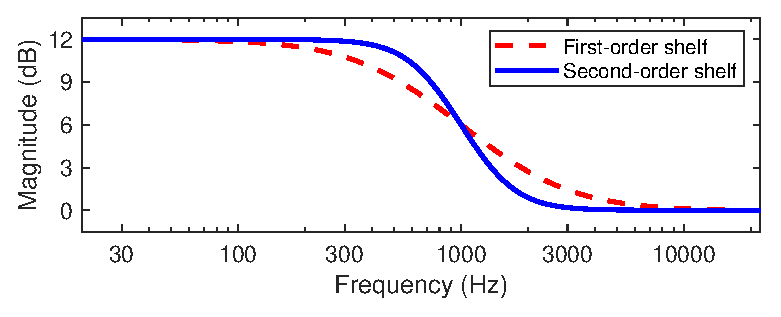
\includegraphics[width=82mm]{fig1_example.eps}
\caption{Figures using color must be understandable also in grayscale printing. It helps if both the line color and the line type are different for each curve.}
\label{fig:example_figure}
\end{figure}

For the final submission photographic and bitmapped images should be submitted as separate JPEG files with a resolution of at least 300 dpi. Line drawings can be submitted in EPS files. The figure number should be clearly indicated in the file name. The size of illustrations when printed in the Journal is usually 82 mm (3.25 inches) wide, although 170 mm (6.75 inches) wide can be used if required. 

Text labels on illustrations must be large enough so that the smallest letters are at least 1.5 mm (1/16 inch) high when the image is reduced to one of the above widths. If possible, text labels on all original illustrations should be scaled so that they will be the same size when reduced for reproduction in the Journal. Figure captions should either be inserted on a separate page of the main manuscript, following the references, or uploaded as a separate file. Captions should be concise.

Figures may publish online in full color; however, they will be converted to grayscale for print. Please review the figures and associated captions and legends/keys to ensure that figures will be understandable after being converted to black and white. For a fee, authors can choose to include color graphics files also in the printed version of the Journal.

\begin{figure*}
\centering
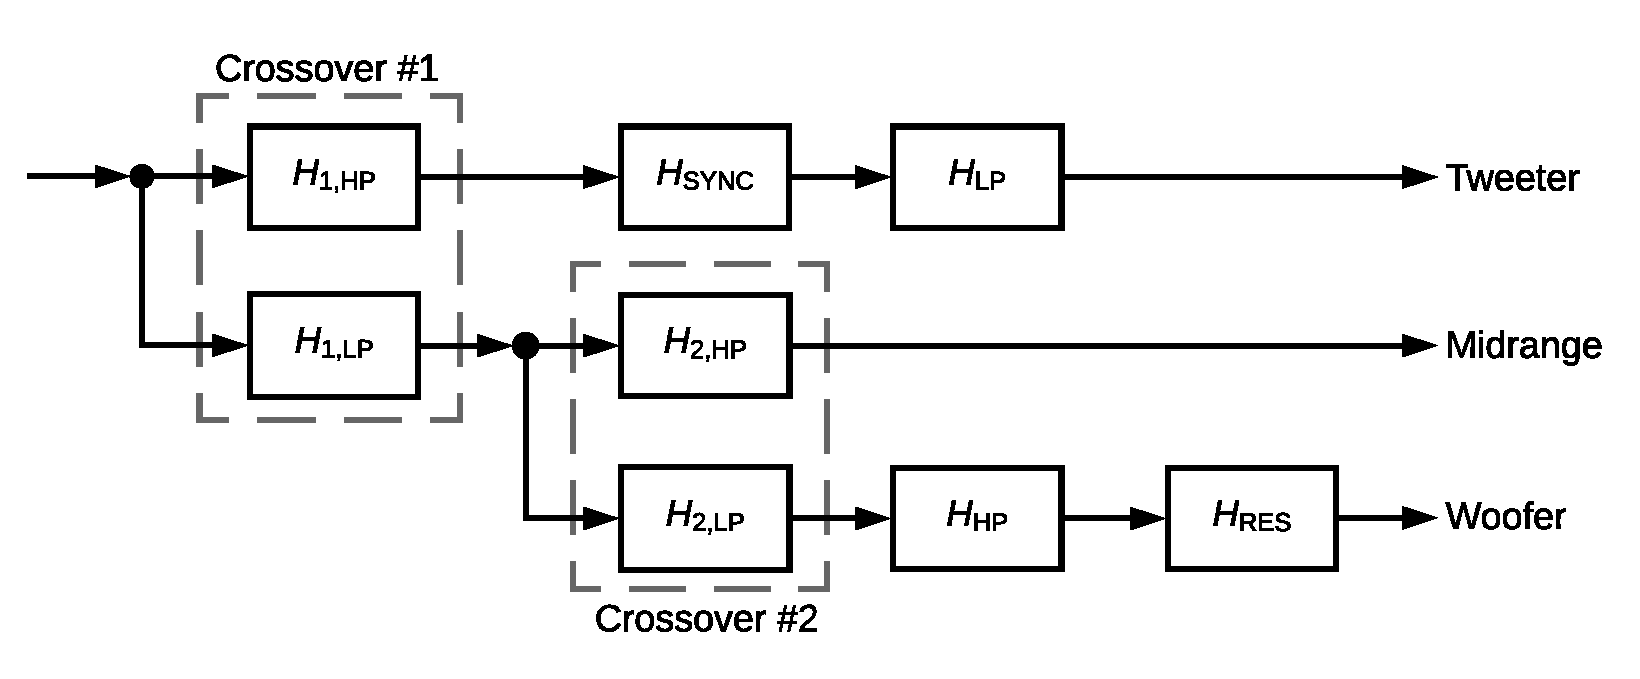
\includegraphics[trim=0cm 0.5cm 0cm 0.5cm, width=0.66\textwidth]{fig2_example.eps}
\caption{Example of a wide figure extending over the two columns.}
\label{wide_figure}
\end{figure*}

\subsection{Tables}

JAES articles often include tables, such as Table \ref{table:an_example_table}. They must be referred to and explained in text. 

%Table
\begin{table}[t]
\tabcolsep8.1pt
\caption{Tables should have a brief caption. Highlighting the best result(s) is helpful to readers.}
\label{table:an_example_table}
{%
\begin{tabular}{@{}lllc@{}}\toprule
Excerpt No.& Genre & Spatial Mode & Correlation\\\colrule
 1 & Pop       & FB   & \textbf{94\%}\\
 2 & Classical & FB   & 33\%\\
 3 & Jazz      & FF   & 76\%\\
 4 & Arabian   & FF   & 41\%\\
 5 & GNE       & H220 & 45\%\\
 6 & GNE       & H45  & 93\%\\
 7 & MNK       & G416 & 74\%\\
 8 & MNK       & D413 & 72\%\\
 9 & MNK       & R420 & \textbf{94\%}\\
10 & MNK       & N516 & 91\%\\\botrule
\end{tabular}}
\begin{tabnote}
Note. This table contains several acronyms which should be defined in the paper, when they are first used (but not in the abstract).
\end{tabnote}
\end{table}

\section{REFERENCE FORMAT AND DOIS}
References should be cited numerically in brackets in order of appearance in the text. References should be listed at the end of the text in order of appearance. In the reference list, please insert “and” between the last and second-to-last author name. Use a comma before “and”, if there are more than two authors in the list. In publication titles, the first letters of the first word and the main words are capitalized in the paper title, but not prepositions and articles (see examples below).

References to periodicals (journals) should include the authors’ names, title of article, periodical title abbreviation, volume, issue number (optional), page numbers or article ID, year and month of publication, and the Digital Object Identifier (DOI) link, if available. The following are examples of the expected format of journal paper references.

\section{CONCLUSION}
The manuscript submitted to JAES should end with a section entitled Conclusion. The Conclusion should briefly review the main points of the paper. However, do not replicate the abstract. All results mentioned in the Conclusion must be deducted from the other parts of the paper. Do not introduce new results in the Conclusion. This section may also speculate on applications and extensions of the results (future work). Many readers browsing technical papers only read the abstract and the Conclusion.

\section{ACKNOWLEDGMENT}
This  work  has  been  funded  in  part  by  the  Academy of   Finland   (project no.~654321). This template version was edited by Kurt James Werner and Vesa V\"alim\"aki. 

%Appendix
\appendix

\section*{APPENDIX}
One or more Appendices can appear after the references. An Appendix can present for example a mathematical derivation, pseudo-code, or other additional data, which is unsuitable to show in the body of the article.

%Biography
 \biography{Matti Meik\"al\"ainen}{headshot1.jpg}{Matti Meik\"al\"ainen is Professor of audio technology at XYZ University, Espoo, Finland. He received his M.Sc. and Ph.D.~degrees from Helsinki University of Technology in 1992 and in 1995, respectively. In 1996, he was a postdoctoral research fellow at the University of Westminster, London, UK. In 2001--2002, he was Professor of signal processing at the Pori School of Technology and Economics, Tampere University of Technology, Pori, Finland. In 2008--2009, he was a visiting scholar at the Center for Computer Research in Music and Acoustics (CCRMA), Stanford University, Stanford, CA. His research interests include musical signal processing, digital filter design, and acoustics of musical instruments. Prof. Meik\"al\"ainen is a senior member of the IEEE and is a member of the Acoustical Society of Finland. He was the Chair of the 11th International Conference on Digital Audio Effects (DAFx), which was held in Espoo, Finland, in 2008.}
 
 \biography{Jane Doe}{headshot2.jpg}{Jane Doe is a Consulting Professor at the Center for Computer Research in Music and Acoustics (CCRMA) in the Music Department at Stanford University where her research interests include audio and music applications of signal and array processing, parameter estimation, and acoustics. She holds Ph.D.~and M.S.~degrees from Stanford University, and an S.B.~from MIT, all in electrical engineering. Dr.~Doe was a researcher at NASA/Ames Research Center, exploring topics in room acoustics and spatial hearing on a grant through the San Jose State University Foundation. She was also chief scientist of Crystal River Engineering, Inc., where she developed their positional audio technology, and a lecturer in the Department of Electrical Engineering at Yale University. Dr.~Doe is a Fellow of the Audio Engineering Society.}
\end{document}
